\documentclass{article}
\usepackage{listings}
\usepackage{graphicx}
\usepackage{float}
\usepackage{amsmath}

\DeclareGraphicsExtensions{.jpg,.png}
\graphicspath{ {/Users/llaryssa/Documents/Stevens/CS532-3DCV/CS532-assignments/assignment7/imgs/} }


\begin{document}

\centerline{\sc \large CS 532: Homework Assignment 7}
\vspace{.2pc}
\centerline{Alana Laryssa Seabra A Santos}
\centerline{\it 12/11/2015}
\vspace{.4pc}

\section{Part b}

For spin images, I'm computing $\beta = dot(n,p_j - p)$ and $\alpha = \sqrt{||p_j - p||^2 - \beta^2}$, where $p$ is the point chosen, $p_j$ are the point cloud points, $n$ is the normal of the point chosen. Then we need to find to which bin allocate the current point, for that I divide $\alpha$ and $\beta$ by the bin size (first normalizing $\beta$ so that I can consider above and below the point chosen).
Below I show a one spin image generated for each $apple_1$ and $banana_1$.

\begin{figure}[ht]
\centering
\begin{minipage}[b]{0.45\linewidth}
  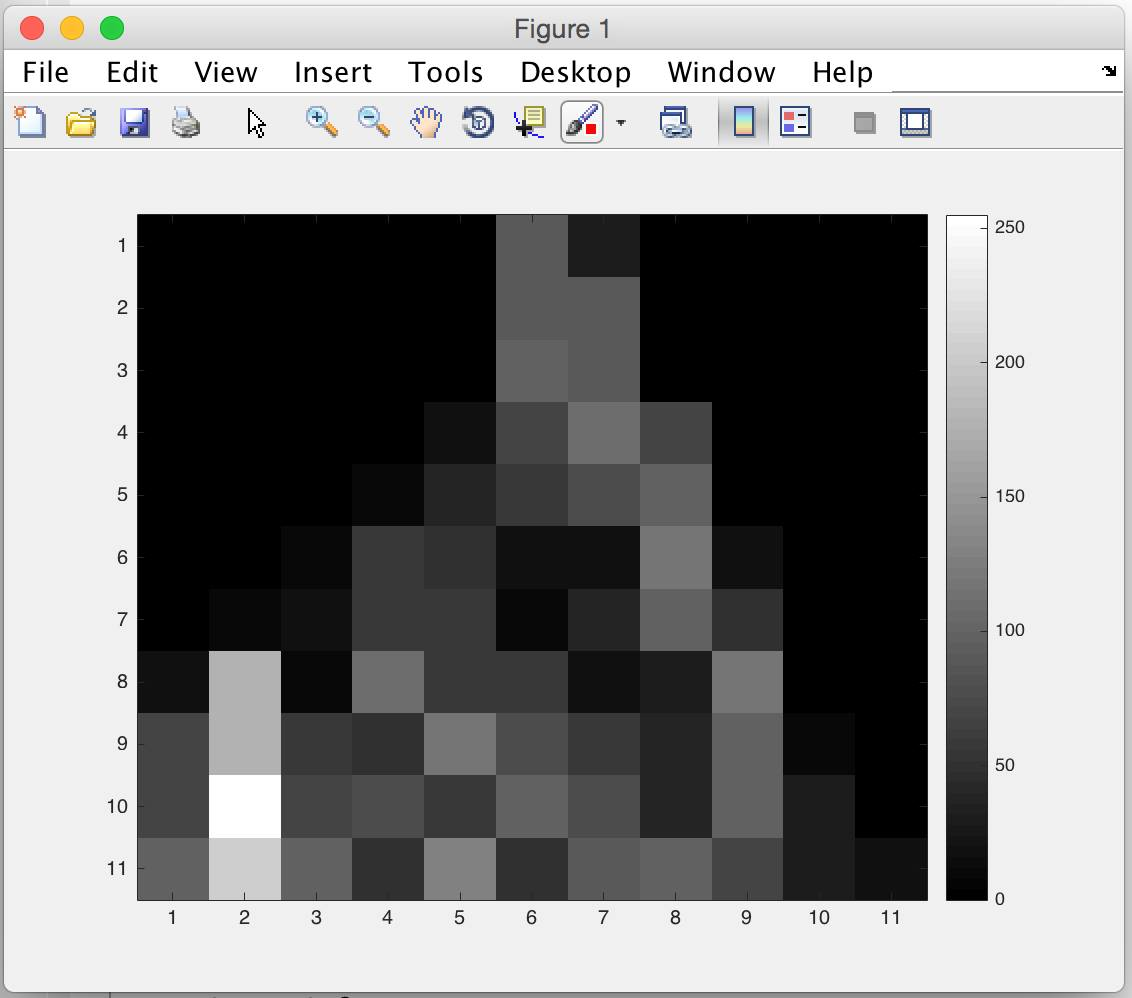
\includegraphics[scale=0.13]{app1}
  \caption{Apple1 Spin Image}
  \label{fig:minipage1}
\end{minipage}
\quad
\begin{minipage}[b]{0.45\linewidth}
  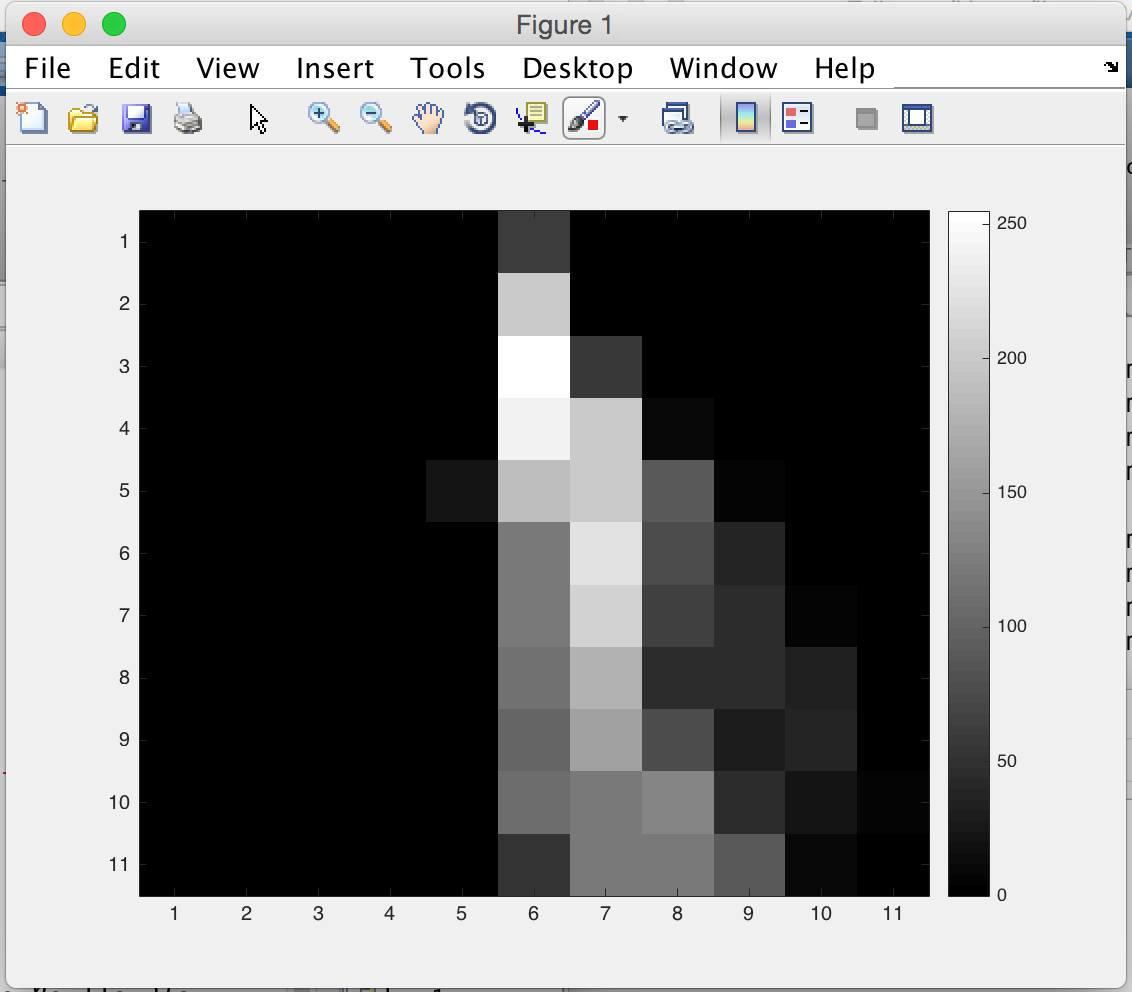
\includegraphics[scale=0.13]{ban1}
  \caption{Banana1 Spin Image}
  \label{fig:minipage2}
\end{minipage}
\end{figure}


\section{Part c}

For the KNN classifier, I'm getting an average of 56.99\% accuracy on 15 runs with different training and test set.
I didn't understand the last part that you say to keep track of correctness of spin image classification. Here is an example of the confusion matrix that I generated when accuracy is 57.77\%:

$confmat = \begin{bmatrix} 9 & 19 & 32 \\ 3 & 54 & 3 \\ 3 & 14 & 43 \end{bmatrix}$

Where "C(i,j) is a count of observations known to be in group i but predicted to be in group j" (from Mathworks).

So we can see that Apple spin images were misclassified most of the time, frequently classified as lemons. And this does not happen in the other way around. Lemons have a reasonable classification accuracy. On the other hand, the algorithm performs really well with Bananas.


\section{Matlab code}

\begin{lstlisting}[language=matlab]

function normals = estimateNormals(obj, sig, k)

    den = 2 * sig^2;

    pts = obj.vertices;
    [idx,dist] = knnsearch(pts, pts, 'k', k);

    normals = [];
    for i = 1:length(pts)
        % compute centroid
        centr = mean(pts(idx(i,:),:));
        % init weights
        w = exp(-dist.^2./den);
        cc = zeros(3,3);
        for j = 1:k
            xj = pts(idx(i,j),:);
            cc = cc + (xj - centr)' * (xj - centr) .* w(i,j);        
        end
        C = cc./sum(w(i,:));
        [V,~] = eig(C);
        normals(i,:) = V(:,1)';
    end

    flip = sign(dot(normals',-pts'))';
    normals = [flip flip flip].*normals;
end


function spin = computeSpinImage(obj, ptidx, nbins, binsize)
    
    if ptidx == 0
        r1 = 1; r2 = length(obj.vertices);
        ptidx = round((r2-r1)*rand+r1);
%         disp(['point idx is: ' num2str(ptidx)]);
    end
    
    spin = zeros(nbins,nbins);
    norml = obj.normals(ptidx,:);
    
    for pt = 1:length(obj.vertices)
        xp = obj.vertices(pt,:) - obj.vertices(ptidx,:);
        
        beta = sum(norml.*xp,2);
        alpha = sqrt(sum(xp.*xp,2) - beta.^2);
    
        % back to zero
        beta = beta - nbins*binsize/2;
        
        b = floor(-beta/binsize) + 1;
        a = floor(alpha/binsize) + 1;
        
        if a > 0 && b > 0 && a <= nbins && b <= nbins
            spin(a,b) = spin(a,b) + 1;
        end
    end
    
    spin = spin(:)';
end


clear all;
% clc;

k = 50;
sig = 20;
knn = 30;

ap1 = readply('hw7/apple_1.ply');
ap2 = readply('hw7/apple_2.ply');
ap3 = readply('hw7/apple_3.ply');
ap4 = readply('hw7/apple_4.ply');

ban1 = readply('hw7/banana_1.ply');
ban2 = readply('hw7/banana_2.ply');
ban3 = readply('hw7/banana_3.ply');
ban4 = readply('hw7/banana_4.ply');

lem1 = readply('hw7/lemon_1.ply');
lem2 = readply('hw7/lemon_2.ply');
lem3 = readply('hw7/lemon_3.ply');
lem4 = readply('hw7/lemon_4.ply');

ap1.normals = estimateNormals(ap1, sig, k);
ap2.normals = estimateNormals(ap2, sig, k);
ap3.normals = estimateNormals(ap3, sig, k);
ap4.normals = estimateNormals(ap4, sig, k);

ban1.normals = estimateNormals(ban1, sig, k);
ban2.normals = estimateNormals(ban2, sig, k);
ban3.normals = estimateNormals(ban3, sig, k);
ban4.normals = estimateNormals(ban4, sig, k);

lem1.normals = estimateNormals(lem1, sig, k);
lem2.normals = estimateNormals(lem2, sig, k);
lem3.normals = estimateNormals(lem3, sig, k);
lem4.normals = estimateNormals(lem4, sig, k);

train = [];
test = [];

cnt = 1;

for i = 1:30   
   train(cnt, :) = [1 computeSpinImage(ap1, 0, 11, 3)];
   train(cnt+1, :) = [1 computeSpinImage(ap2, 0, 11, 3)];
   train(cnt+2, :) = [2 computeSpinImage(ban1, 0, 11, 3)];
   train(cnt+3, :) = [2 computeSpinImage(ban2, 0, 11, 3)];
   train(cnt+4, :) = [3 computeSpinImage(lem1, 0, 11, 3)];
   train(cnt+5, :) = [3 computeSpinImage(lem2, 0, 11, 3)];
   
   test(cnt, :) = [1 computeSpinImage(ap3, 0, 11, 3)];
   test(cnt+1, :) = [1 computeSpinImage(ap4, 0, 11, 3)];
   test(cnt+2, :) = [2 computeSpinImage(ban3, 0, 11, 3)];
   test(cnt+3, :) = [2 computeSpinImage(ban4, 0, 11, 3)];
   test(cnt+4, :) = [3 computeSpinImage(lem3, 0, 11, 3)];
   test(cnt+5, :) = [3 computeSpinImage(lem4, 0, 11, 3)];
   
   cnt = cnt+6; 
end

train_lbl = train(:,1);
train_data = train(:,2:end);

test_lbl = test(:,1);
test_data = test(:,2:end);

correct = 0;


for i = 1:size(test,1)
    sample = test_data(i,:);
    idx = knnsearch(train_data, sample, 'K', knn); 
    votes = zeros(3,1);
    for j = 1:knn
       votes(train_lbl(idx(j))) = votes(train_lbl(idx(j))) + 1;
    end
    
%     [~,lbl] = max(votes);
%     if lbl == test_lbl(i)
%         correct = correct + 1;
%     end 

    [vv, labels] = sort(votes, 'descend');
    
    if all(vv==vv(1)) % all the same
        if labels(1) == test_lbl(i)
            correct = correct + 0.33;
        end
    elseif vv(1)==vv(2)
        if labels(1) == test_lbl(i)
            correct = correct + 0.5;
        end
    else
        if labels(1) == test_lbl(i)
            correct = correct + 1;
        end
    end
    
    knnout(i) = labels(1);   
end

disp(['accuracy: ' num2str(correct/size(test_data,1))])
confmat = confusionmat(test_lbl,knnout')


















\end{lstlisting}


\end{document}



